%!TEX root = ../report.tex
\chapter{Introduction}
\label{cha:Introduction}
In computer science, graphs are structures used for representing relationships between objects. Most information is related to other pieces of information and by using these inherent relations a graph can be created. By ordering information in a graph structure it can considered a ``knowledge graph''. When creating knowledge graphs a standard called ``Resource Description Framework'' (RDF) is commonly used. RDF was created to be a common machine-readable standard for use on the web. In RDF data is stored as triples, where a triple has the structure ``subject-predicate-object''. Comparing this structure to other graphs, the subject and object is the same as vertices in the graph, and the predicate is a directed edge. In addition to forming the relation between the two vertices, the predicate also holds a type of relation. This makes it possible to apply reason to the data set and derive new information from what is already there. An example of the RDF structure can be seen in figure \ref{fig:spatiotemporalTrondheim}, with Trondheim as the central vertex, connected to spatial and temporal data, and displaying a place hierarchy.

\begin{figure}[h]
  \centering
  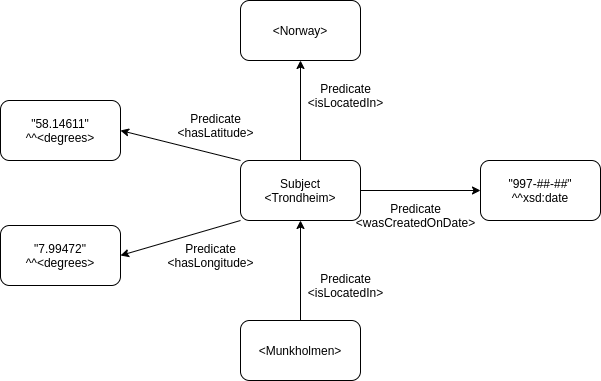
\includegraphics[scale=0.5]{figs/rdfSPO.png}
 \caption{Trondheim with spatiotemporal data}
 \label{fig:spatiotemporalTrondheim}
\end{figure}

There are a few projects using RDF as an information storage system. Some of the more well-known are DBPedia\cite{dbpedia}, YAGO\cite{yago}, and Creative Commons. Both DBPedia and YAGO consist of a large linked data set, while Creative Commons use RDF for embedding licenses. YAGO and DBPedia contain spatial and temporal data, making both suited for applications related to time and space. Because RDF is machine readable this data is suited for use in many different aspects of computer science, but it requires knowledge of the underlying structure of the data. By creating methods that allows for more human accessible information from RDF data, the format can be used without a deep understanding of the graph and makes it possible to create applications with utility.

Storing large graph structures requires specialized storage methods. With RDF a commonly used storage method is the triple storage. There have also been created special databases for graphs. Comparing such graph storage to relational storage, graph storage generally outperforms relational storage on structural queries, but not on data queries \cite{AComparisonOfGraphAndRelDB}. Structural queries reference the graph structure, or the relationships in the data, while data queries look for specific data. When creating a graph database, an indexing system can also be added. Such a system is Neo4j\footnote{https://neo4j.com/} that use Apache Lucene\footnote{https://lucene.apache.org/} for indexing.

When using graphs as a form of storage, the vertices hold data, and the edges can be given an extra property describing the relation. Combining such data storage with common traversal methods for graphs results in an efficient extraction model for relational data. Some common traversal methods include breadth first search, where all neighboring vertices are discovered before moving on to the children of the currently discovered vertices. This contrasts to depth first search, where the children of a vertex are visited as they are discovered. In this thesis methods for efficient keyword search on spatial and temporal data will be explored.

\section{Background and motivation}
\label{sec:BackgroundAndMotivation}
Most of the information on the web is unstructured, or semi-structured data. Using metadata and automated processes to create structures can help both humans and computers to find new uses for this information. Making the information in RDF more accessible can creating new applications and makes it possible to create more utility from existing data sets. To be able to get more utility out of RDF, it needs to be more accessible for humans. As more data is generated, there are also more relations between the data. Exploring these relations can be done by using RDF or other graphs, but for a regular person this can be difficult. By showing that fast and accurate keyword search of spatiotemporal RDF graphs is possible new utilities can be created.

\section{Goals and research questions}
\label{sec:Goals and Research Questions}
\begin{description}
    \item[Goal] {\em This thesis has the goal of researching methods for spatiotemporal keyword searches on large RDF graphs, and finding aspects needs to be considered for speed and accuracy.}
\end{description}
Accomplishing this goal proves that RDF graphs can be used as a tool for structuring spatial and temporal data. There is a lot of data that can be placed at one or more real locations, either directly, or indirectly. By using RDF graphs, it is possible to model how different places are connected through data, and how different pieces data can be related to real places. This is also extended to time, meaning that RDF graphs can model how time relates to other data.

\begin{description}
    \item[Research question 1] {\em How can spatiotemporal data be integrated into existing keyword query methods for RDF data?}
\end{description}
Extending existing methods for searching RDF data can make it simpler to search spatiotemporal data. By combining methods for temporal and spatial search, methods for spatiotemporal search should be possible to research.

\begin{description}
    \item[Research question 2] {\em What methods can be used to achieve greater speed and accuracy for searches on RDF data?}
\end{description}
An important aspect of any search is speed and accuracy. Since searching in graphs usually entails some form of traversal, the methods of traversal, as well as factors that affect speed and accuracy will be researched.

\begin{description}
    \item[Research question 3] {\em How do spatial and temporal RDF query methods differ from other query methods?}
\end{description}
Comparing spatial, temporal and spatiotemporal searches can tell how spatiotemporal data differs in RDF graphs. This is important so that optimized methods can be developed.

\section{Research method}
\label{sec:researchMethod}
This thesis will build on previous keyword search approaches for RDF graphs and determine what methods can be expanded to incorporate spatiotemporal queries. A method for spatiotemporal search will be created, and methods for improvement will be tested, with the goal of finding what aspects of the search method have most effect for speed and accuracy. Comparing spatial, temporal, and spatiotemporal searches using time and accuracy as metrics, will give insight into how the data differs, and how searching can be optimized.

\glsresetall